\documentclass[a4paper, 10pt]{RelazioneLab}

\title{Relazione contatore a due cifre}
\author{Scapin Alessandro - Gruppo Greco/Scapin}
\date{17 Maggio 2024}

\headerleft{Scapin Alessandro} % Left running head
\headerright{Contatore a due cifre} % Right running head: Student ID and Name
\footertext{} % Text to appear in the footer, leave this command empty for no footer text

\begin{document}

\maketitle

\section{Materiale}
\begin{multicols}{2}
    \begin{itemize}
        \item Breadboard
        \item DIP-Switch x 8 | G\&K SDA08
        \item Display 7 segmenti rosso a catodo comune
        \item Cavetti rigidi
        \item CD4518
        \item CD4511
    \end{itemize}
\end{multicols}
\section{Riferimenti teorici}
\subsection{Contatore}
Il contatore è un dispositivo elettronico in grado di eseguire il compito di contare. Viene costruito con dei dispositivi in grado di memorizzare dati, flip-flop e, può essere sincrono nel caso in cui il clock di tutti i flip-flop di cui è composto siano collegati insieme o asincrono nel caso in cui il clock di quest'ultimi non sia collegato direttamente al clock del segnale. Il modulo del contatore rappresenta quanti numeri "utilizza" il contatore: nel nostro caso 1000.
\subsection{Display 7 segmenti}
Il display a 7 segmenti è un display in grado di mostrare una cifra grazie a 7 sette segmenti led che si accendono in maniera tale da formare il numero desiderato. Questi display possono essere pilotati da dei circuiti integrati così da comandarli direttamente con un codice BCD. Oltre al colore, che può variare, un'importante caratteristica di questi display è il pin in comune con tutti i led, il catodo o l'anodo.
\subsection{Segnale di clock}
Il segnale di clock è un segnale periodico, nel nostro caso un'onda quadra, che varia nel tempo e permette l'avanzamento dei numeri sul display.
\section{Procedimento}
    \begin{enumerate}
        \item Descrivere dettagliatamente il problema; una volta fatto ciò si andrà a determinare i componenti necessari per assemblare il circuito.
        \item Disegnare lo schema logico utilizzandolo poi per ricavare lo schema di montaggio su breadboard. È consigliabile progettare quest'ultimo prima di iniziare l'assemblaggio in maniera tale da posizionare sin da subito i componenti nella posizione ottimale.
        \item Inziare ad assemblare i componenti sulla breadboard avendo cura di utilizzare i colori rosso e nero solo per l'alimentazione, piegando i cavi in modo tale da formare solo angoli retti e evitando di passare sopra gli integrati. 
        \item Una volta che ci si è assicurati del corretto funzionamento del circuito tramite il generatore di funzioni, è possibile sostituire il generatore di funzioni con, ad esempio, una fotocellula che darà un colpo di clock quando un oggetto ci passa davanti.
        \item Attivando lo switch S1 il contatore viene resettato mentre attivando lo switch S2 viene attivato o disattivato il conteggio. 
        \item Chiedere al docente di laboratorio l'autorizzazione per il collaudo del circuto.
        \item Eseguire il collaudo prestando attenzione a verificare tutte le possibili combinazioni possibili; nel caso in cui ci siano delle incongruenze si può ricorrere a un tester per controllare la correttezza delle tensioni o verificare la continuità dei conduttori.
        \item \item Descrivere dettagliatamente il problema; una volta fatto ciò si andrà a determinare i componenti necessari per assemblare il circuito.
        \item Disegnare lo schema logico utilizzandolo poi per ricavare lo schema di montaggio su breadboard. È consigliabile progettare quest'ultimo prima di iniziare l'assemblaggio in maniera tale da posizionare sin da subito i componenti nella posizione ottimale.
        \item Inziare ad assemblare i componenti sulla breadboard avendo cura di utilizzare i colori rosso e nero solo per l'alimentazione, piegando i cavi in modo tale da formare solo angoli retti e evitando di passare sopra gli integrati. 
        \item Una volta che ci si è assicurati del corretto funzionamento del circuito tramite il generatore di funzioni, è possibile sostituire il generatore di funzioni con, ad esempio, una fotocellula che darà un colpo di clock quando un oggetto ci passa davanti.
        \item Attivando lo switch S1 il contatore viene resettato mentre attivando lo switch S2 viene attivato o disattivato il conteggio. 
        \item Chiedere al docente di laboratorio l'autorizzazione per il collaudo del circuto.
        \item Eseguire il collaudo prestando attenzione a verificare tutte le possibili combinazioni possibili; nel caso in cui ci siano delle incongruenze si può ricorrere a un tester per controllare la correttezza delle tensioni o verificare la continuità dei conduttori.
        \item \item Descrivere dettagliatamente il problema; una volta fatto ciò si andrà a determinare i componenti necessari per assemblare il circuito.
        \item Disegnare lo schema logico utilizzandolo poi per ricavare lo schema di montaggio su breadboard. È consigliabile progettare quest'ultimo prima di iniziare l'assemblaggio in maniera tale da posizionare sin da subito i componenti nella posizione ottimale.
        \item Inziare ad assemblare i componenti sulla breadboard avendo cura di utilizzare i colori rosso e nero solo per l'alimentazione, piegando i cavi in modo tale da formare solo angoli retti e evitando di passare sopra gli integrati. 
        \item Una volta che ci si è assicurati del corretto funzionamento del circuito tramite il generatore di funzioni, è possibile sostituire il generatore di funzioni con, ad esempio, una fotocellula che darà un colpo di clock quando un oggetto ci passa davanti.
        \item Attivando lo switch S1 il contatore viene resettato mentre attivando lo switch S2 viene attivato o disattivato il conteggio. 
        \item Chiedere al docente di laboratorio l'autorizzazione per il collaudo del circuto.
        \item Eseguire il collaudo prestando attenzione a verificare tutte le possibili combinazioni possibili; nel caso in cui ci siano delle incongruenze si può ricorrere a un tester per controllare la correttezza delle tensioni o verificare la continuità dei conduttori.
    \end{enumerate}
\section{Schemi}
\begin{figure}[H]
    \centering
    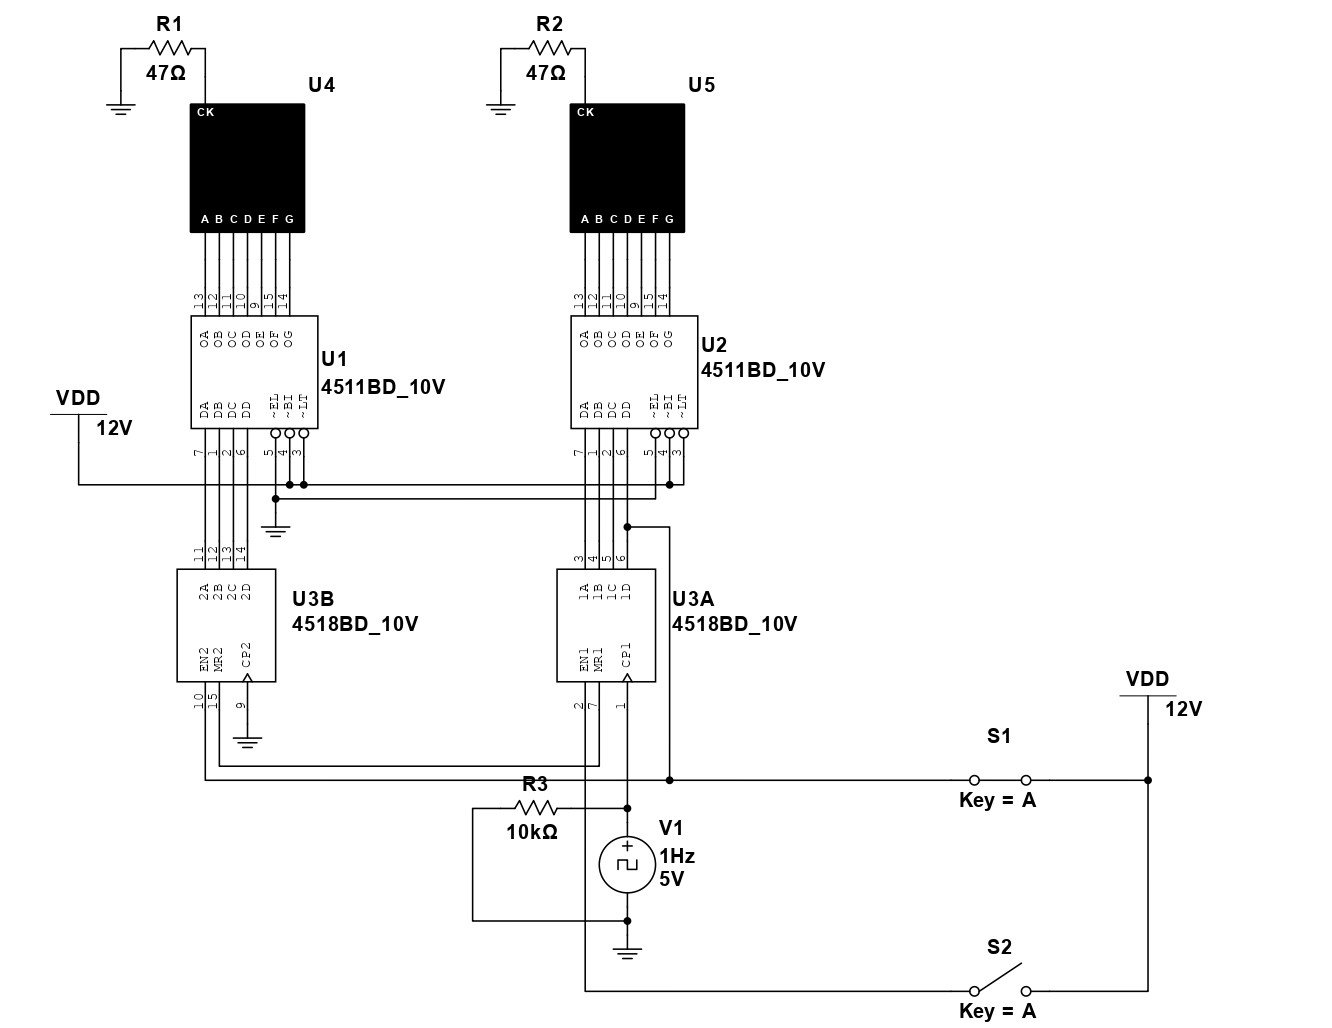
\includegraphics[width=0.8\textwidth]{schema_page-0001.jpg}
    \caption{Schema funzionale}
    \label{fig:enter-label}
\end{figure}
\begin{figure}[H]
    \centering
    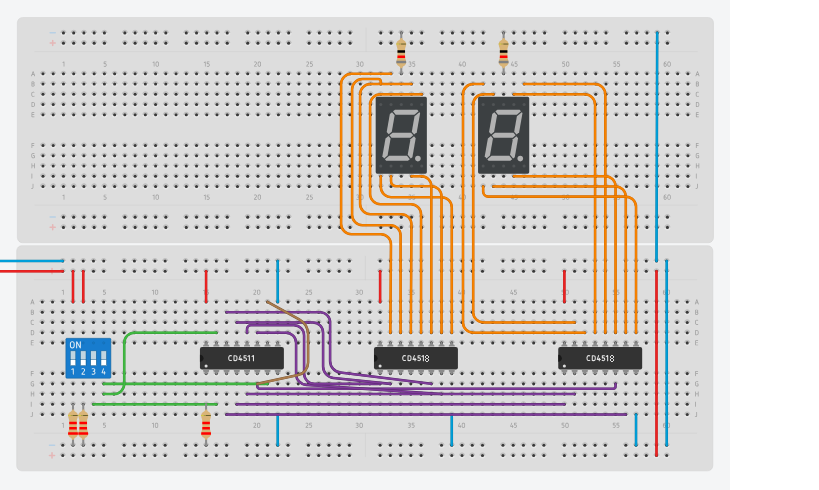
\includegraphics[width=0.8\textwidth]{BIMBIMBBAMBAM.png}
    \caption{Schema di montaggio}
    \label{fig:enter-label}
\end{figure}
\section{Conclusioni}
Il circuito inizialmente presentava dei difetti dovuti principalmente ad un 4518 difettoso; una volta individuato il problema e sostituendo il seguente integrato abbiamo risolto questo difetto. Fatto ciò tutto il circuito funzionava correttamente. Inoltre abbiamo anche sostituito il generatore di funzioni con una fotocellula per far avanzare il conteggio ogni qualvolta si presentasse un oggetto davanti alla fotocellula. 
\end{document}